\documentclass[12pt]{article}
\usepackage[a4paper, total={6in, 9in}]{geometry}
\usepackage{graphicx}
\graphicspath{ {./images/output/} }
\usepackage{caption}
\usepackage[english]{babel}
\usepackage{titling}
\usepackage{float}
% \usepackage{amsmath}
% \usepackage{minted}
% \usepackage{multicol}
% \usepackage{array}
% \usepackage{setspace}
% \usepackage{placeins}
% \usepackage{hyperref}
\setlength{\parindent}{0pt}

% \usepackage{lipsum}

\title{Drawing Line Diagrams in AutoCAD Electrical.}
\author{}
\date{}

\pagenumbering{gobble}
\begin{document}
\vspace*{\fill}
\begin{center}

    \emph{Heaven's Light is Our Guide} \\
    \textbf{Rajshahi University of Engineering and Technology} \\

    \begin{figure}[H]
        \centering
        
\includegraphics[scale=.34]{images/RUET_logo.png}
        \label{fig:ruet_logo}
    \end{figure}
    \vspace{5mm}

    \textbf{Course Code}\\
    ECE 3200\\
    \vspace{3mm}
    \textbf{Course Title}\\
    Electrical Services Design

    \vspace{5mm}
    \textbf{Experiment Date:} {February 4, 2025}\\
    \textbf{Submission Date:} {February 18, 2025}\\

    \vspace{5mm}
    \textbf{Lab Report 5: \\ Implementation of Parametric \& Full Units PLC: Insertion, Editing, \& Modification.}

    \vspace{15mm}

    \begin{tabular}{c|c}
        \textbf{Submitted to} & \textbf{Submitted by} \\
        Md. Faysal Ahamed     &                       \\
        Lecturer              &                       \\
        Dept of ECE, RUET     & Md. Tajim An Noor     \\
        -                     & Roll: 2010025         \\
        Moloy Kumar Ghosh     &                       \\
        Lecturer              &                       \\
        Dept of ECE, RUET     &                       \\
    \end{tabular}

\end{center}
\vspace*{\fill}


\pagebreak

\tableofcontents

\pagebreak
\pagenumbering{arabic}
\maketitle

\section*{Introduction}
\addcontentsline{toc}{section}{Introduction}
In this experiment, forward and reverse contactor diagrams were created using AutoCAD Electrical. These diagrams are crucial for controlling motors in industrial applications, allowing for the switching of motor rotation direction \cite{motor_control}. The process began with understanding the basic concepts and functionality of forward and reverse contactors \cite{contactor_basics}, which was essential for accurate diagram design.
\\\\
The experiment utilized various tools within AutoCAD Electrical, such as the symbol library, drawing shortcuts, and wiring commands \cite{autocad_tools}. Mastery of these tools ensured precision and efficiency. Additionally, best practices for electrical drawing were followed, including clarity, standard symbols, and proper labeling \cite{electrical_drawing}, which are vital for effective communication among engineers and technicians.
\\\\
The objective of the experiment was to gain a comprehensive understanding of how to effectively use AutoCAD Electrical for creating functional electrical diagrams. By connecting theoretical knowledge with practical applications, the experiment aimed to enhance proficiency in electrical drawing and circuit design, ultimately preparing participants for real-world engineering challenges.

\section*{Required Equipment/Software}
\addcontentsline{toc}{section}{Required Equipment/Software}
\begin{itemize}
    \item AutoCAD Electrical
    \item \LaTeX{} for report writing
\end{itemize}

\section*{Procedure}
\addcontentsline{toc}{section}{Procedure}
\begin{enumerate}
    \item Open AutoCAD Electrical and create a new project.
    \item Insert a new drawing into the project.
    \item Insert a 3-phase vertical ladder in the schematic.
    \item Draw two horizontal lines from the ladder using the multiple bus tool.
    \item Insert a 3-phase motor at the end of the first horizontal bus.
    \item Add fuses and magnetic contactors to both horizontal buses.
    \item Add an overload relay to the first bus.
    \item Format the drawing with appropriate colors and labels.
    \item Edit the wires using trim and stretch tools.
    \item Verify the diagrams for accuracy.
    \item Save the drawings and project.
\end{enumerate}


\begin{figure}[H]
    \centering
    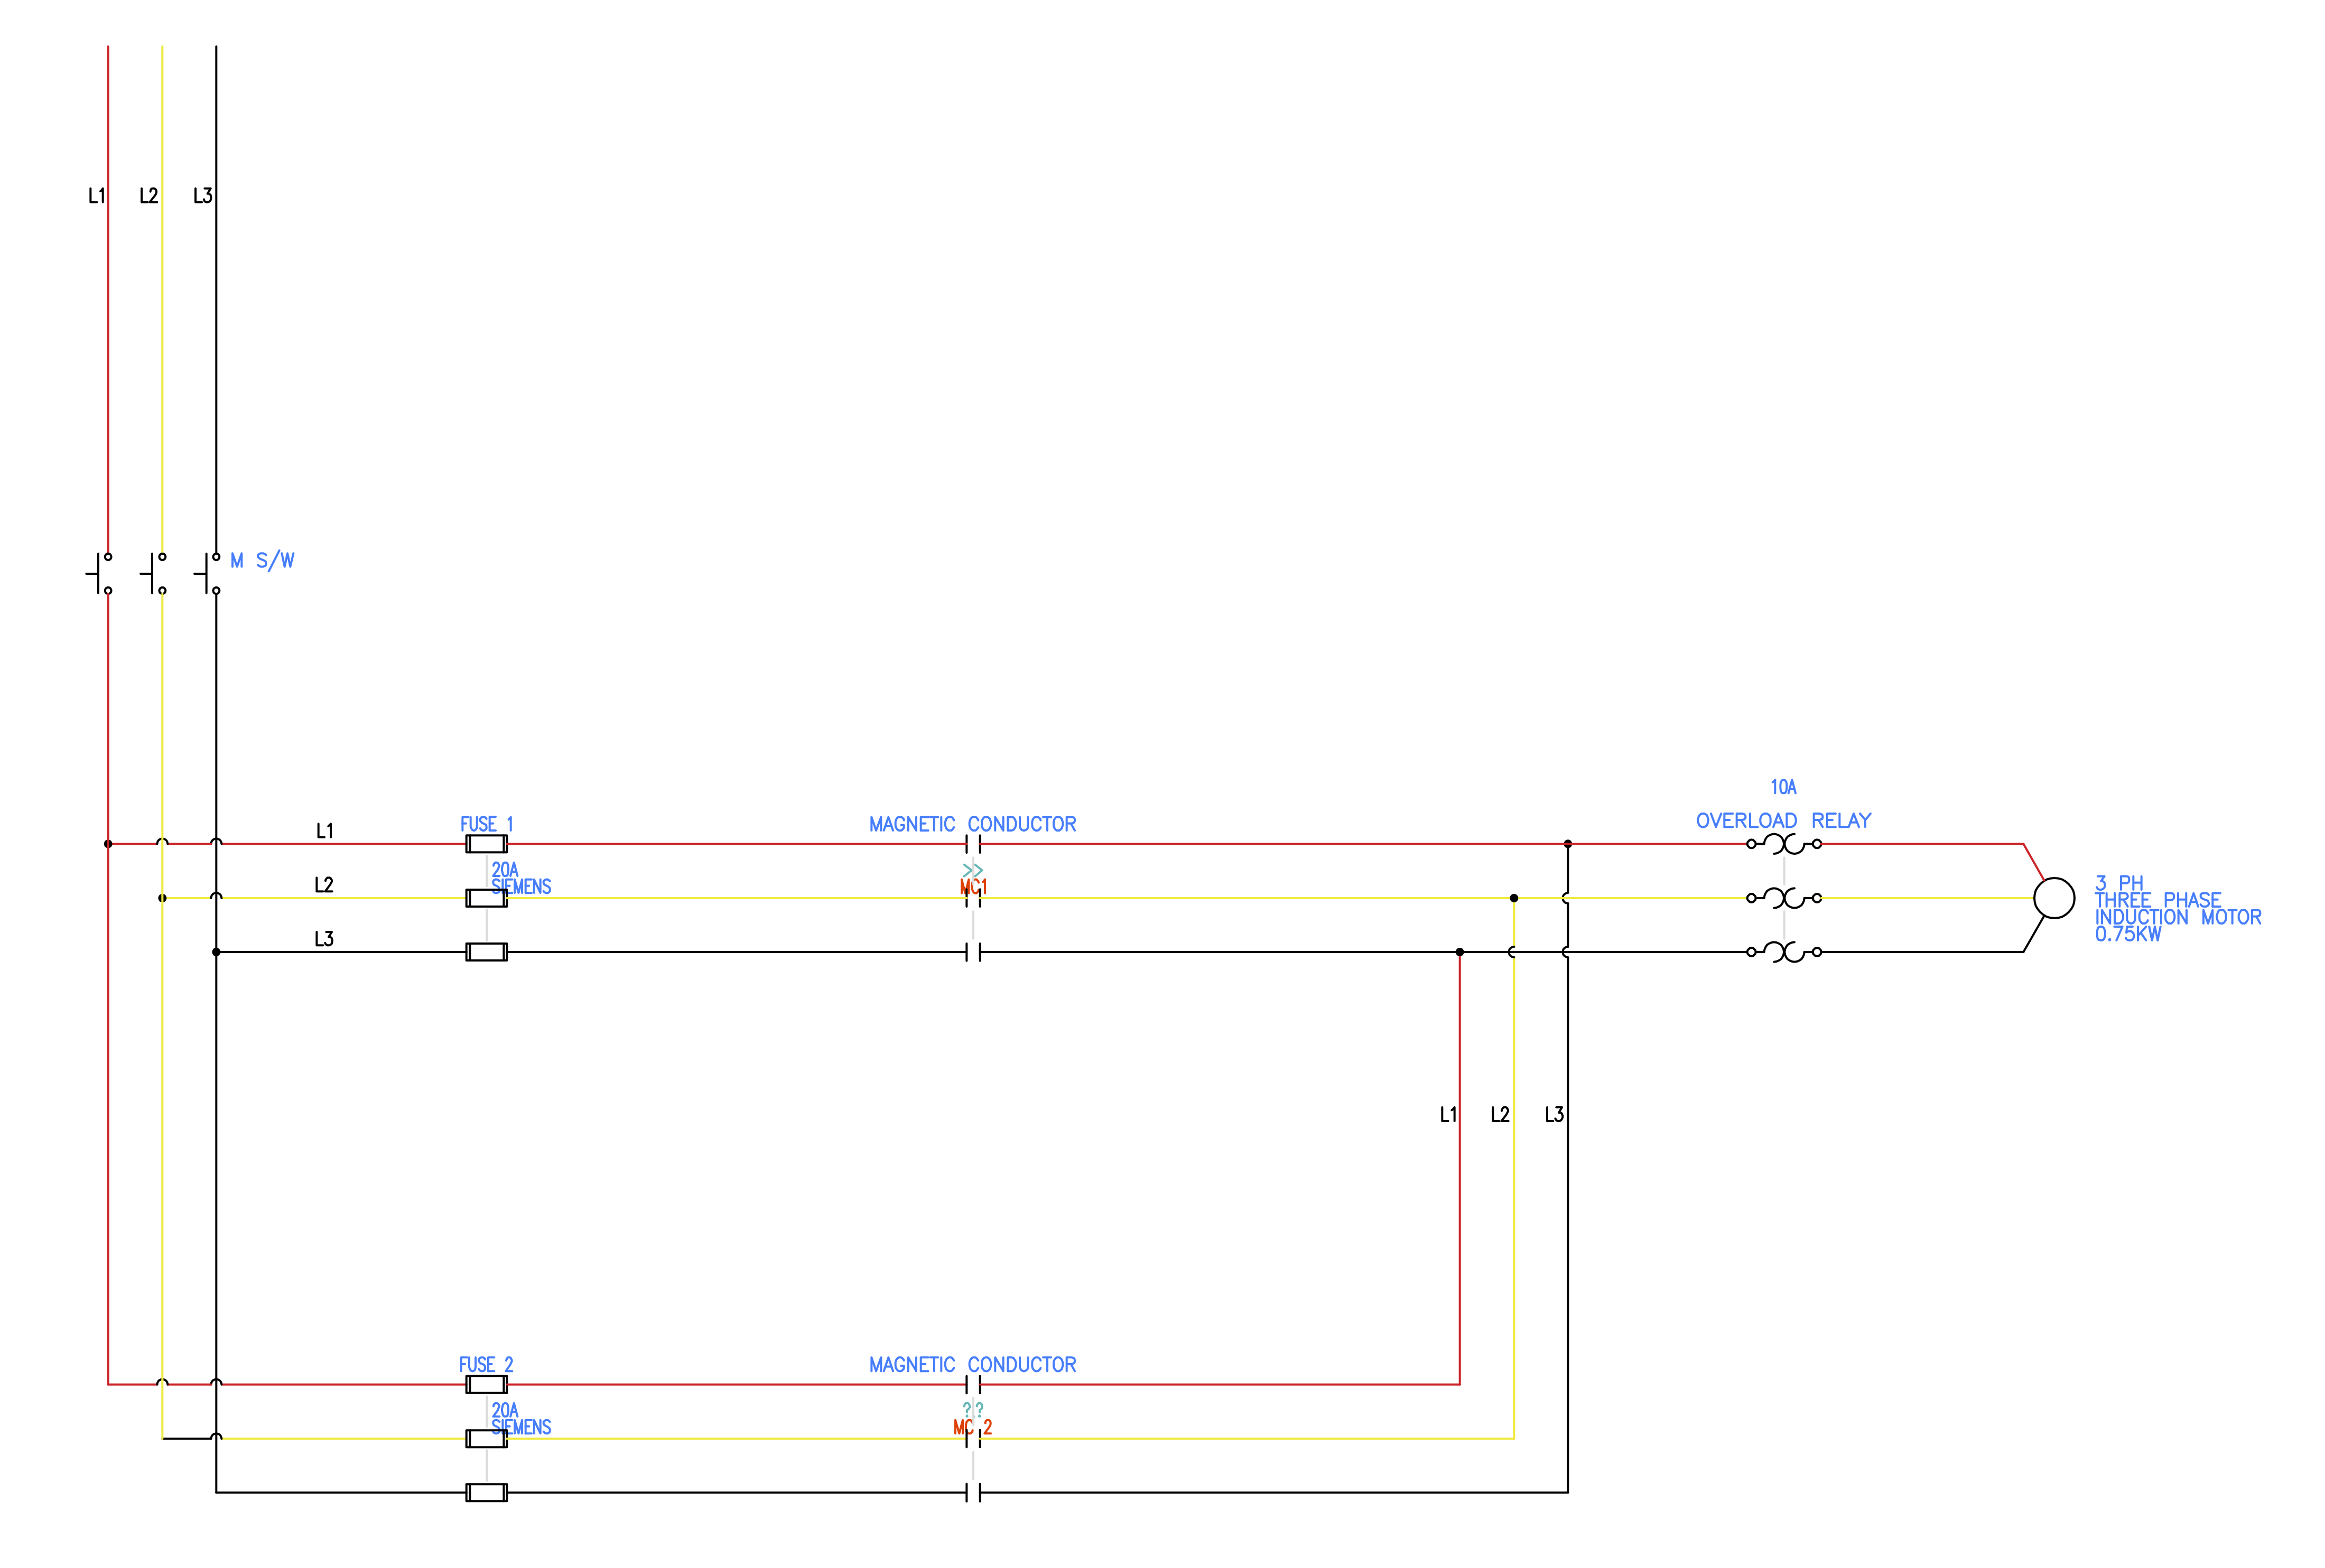
\includegraphics[width=\textwidth]{1.png}
    \caption{Inserting Parametric \& Full unit PLC}
    \label{fig:insert}
\end{figure}


\section*{Discussion \& Conclusion}
\addcontentsline{toc}{section}{Discussion \& Conclusion}
The experiment demonstrated the creation of forward and reverse contactor diagrams using AutoCAD Electrical. The outlined procedure ensured accurate construction, showcasing motor direction control in industrial applications. AutoCAD Electrical's tools, like the symbol library and wiring commands, streamlined the process.
\\\\
Understanding forward and reverse contactors was crucial for correct diagram design. Adhering to best practices in electrical drawing, such as clarity, standard symbols, and proper labeling, is vital for effective communication.
\\\\
In conclusion, the experiment provided valuable insights into using AutoCAD Electrical for functional electrical diagrams, enhancing skills applicable to real-world engineering challenges.
\\\\
The experiment is done following these video:\\
AutoCAD Electrical Bangla Tutorial Class - 14 How to Inserting Parametric \& Full Units PLC (https://youtu.be/AoIb3zPTxdc?si=ezYcLeiw5AbrGDLT)


\bibliographystyle{IEEEtran}
\renewcommand{\bibname}{References}
\addcontentsline{toc}{section}{References}
\bibliography{ref}

\end{document}
